% -*- root: diplomarbeit.tex -*-
\section{Einleitung}
\textbf{Computer Vision}, das machinelle Sehen, ist eine große Herausforderung in der Bildverarbeitung und Feld intensiver Forschung. Die zunehmende Leistungsfähigkeit der Rechner und verbesserte Qualität auch preiswerter Kameratechnik in den letzten Jahren intensivieren die Bestrebungen auf diesem Gebiet zusätzlich. Die dadurch entstandenen Ansätze, Modelle und Methoden haben längst in vielen Bereichen des Alltags Einzug gehalten. Kaum ein Auto wird ohne intelligente Sensorik ausgestattet und unterstützt den Fahrer beispielsweise durch Lesen von Straßenschildern, Erkennen von Fahrbahnmarkierungen sowie Fußgängern oder anderen Verkehrsteilnehmern \cite{PED}. Die Industrie nutzt computergesteuerte Auswertungen von Kamerabildern zur Qualitätssicherung von Bauteilen wie zum Beispiel Displays \cite{LCD}. In der Medizin helfen computergestützte visuelle Verfahren bei der Analyse von Bilddaten und unterstützen so die Diagnostik \cite{MIP}. Und nicht zuletzt bildet die Auswertung von Kameradaten auch im Forschungsbereich der Robotik die Grundlage für viele unterschiedliche Anwendungen. Die Aufgaben, die an den Bereich Computer Vision gestellt werden, sind somit vielfältig.

Diese Arbeit behandelt einen speziellen Teilbereich des maschinellen Sehens: das Finden (Detection) und Verfolgen (Tracking) von Objekten. Ein definiertes Objekt, das in einer bestimmten Art und Weise repräsentiert ist, soll somit in einem Bild gefunden und verfolgt werden. Da noch nicht verstanden ist, wie das Gehirn visuelle Daten zur Erkennung von ``gelernten'' Objekten verarbeitet, ist eine Adaption auf Computerebene nicht möglich. Die Natur kann also nicht vollkommen als Vorbild dienen. Aus diesem Grund wurden im Laufe der letzten Jahrzehnte unterschiedliche Ansätze entwickelt, die mittlerweile sehr gute Ergebnisse liefern, sich allerdings oft auf einen Teilbereich oder ein spezielles Szenario beschränken.

Neben der algorithmischen Lösung der Objekterkennung treten zudem eine Reihe technischer Herausforderungen auf, die beinahe jeder Tracking-Detection-Ansatz zumindest teilweise bewältigen muss:

\begin{itemize}
\item Informationsverlust durch Projektion der 3D-Welt in 2D-Bilder,
\item Bildrauschen,
\item Komplexe Bewegungen des Objekts,
\item Teilweises oder komplettes Verdecken des Objekts,
\item Änderungen in der Belichtung der Szene,
\item Bewegungen der Kamera,
\item etc.
\end{itemize}

Umwelteinflüsse und technische Einschränkungen spielen somit eine große Rolle für den Erfolg des machinellen Sehens.\cite{OTS}.

Die Wahl der richtigen beziehungsweise geeignetsten Bildverarbeitungsmethoden richtet sich nicht zuletzt auch nach dem Einsatzgebiet der Implementation. Zusätzlich hat es auch Einfluss auf die Komplexität der Lösung. Eine statische Überwachungskamera, die Bewegungen registrieren soll, bietet beispielsweise eine softwaretechnisch relativ simple Lösung. Da sie permanent den gleichen Hintergrund aufnimmt, kann durch simple Subtraktion zweier Folgebilder eine robuste Objekterkennung erfolgen. Das Erkennen von bestimmten Objekten wie Gesichtern, Straßenschildern oder Produktionsfehlern benötigt wiederum andere, komplexere Methoden, da die Spezifität des Objekts selbst eine Rolle spielt. Manche Aufgabenstellungen sind mittlerweile gut und zufriedenstellend zu lösen, andere hingegen stellen weiterhin eine große Herausforderung dar. Die in Kapitel \ref{section_2} vorgestellten Paradigmen begegnen den Problemen auf unterschiedliche Arten und Weisen.

\subsection{Zielsetzung dieser Arbeit}
In dieser Arbeit wird ein Tracking-Detection Algorithmus in C++ implementiert und auf seine Tauglichkeit für das Erkennen von Flugrobotern wie Quadro- oder Hexakoptern getestet. Diese sollen sich gegenseitig mittels eines Kamerabildes erkennen können, um entsprechende autonome Handlungen auszuführen. Dabei gibt es eine Reihe von Restriktionen, die eingehalten werden müssen.

Die Kopter erhalten keine zusätzlichen Komponenten wie Leuchtdioden beziehungsweise spezielle Farb- oder Musterapplikationen zur Identifizierung. Jeder Kopter soll seine Individualität durch sich selbst ausdrücken und so zu identifizieren sein. Das Detektieren der Kopter soll unter realen Bedingungen funktionieren. Umwelteinflüsse, Veränderungen der Lichtverhältnisse etc. müssen dem-entsprechend behandelt und gefiltert werden. Daten aus unterstützende Systemen zur Lokalisierung der Kopter, zum Beispiel GPS oder anderen Ortungssystemen, stehen ebenfalls nicht zur Auswertung zur Verfügung. Zusätzlich soll die Verarbeitung in Echtzeit erfolgen, weil die Ergebnisse direkt Einfluss auf die Navigation der Flugroboter haben.

Diese Vorgaben schränken die Wahl der Methoden stark ein. Algorithmen, die zum Beispiel allein auf die Verarbeitung von Farbwerten basieren, können nicht in Betracht gezogen werden, da Umwelteinflüsse das Ergebnis leicht verfälschen können.

Deshalb wurde zur Umsetzung der \textit{TLD - Tracking-Learning-Detection} \cite{TLD} als Algorithmus gewählt. TLD findet beliebige Objekte in einem Bild, benötigt keine speziellen Initialisierungsmechanismen oder Lernphasen, ist leicht verständlich und gut zu implementieren. Das allgemeine Verarbeitungsschema ist in Abbildung \ref{TLD-Schema} dargestellt. Die Details werden in Kapitel \ref{section_3} im Einzelnen erläutert.

\begin{figure}
\centering{}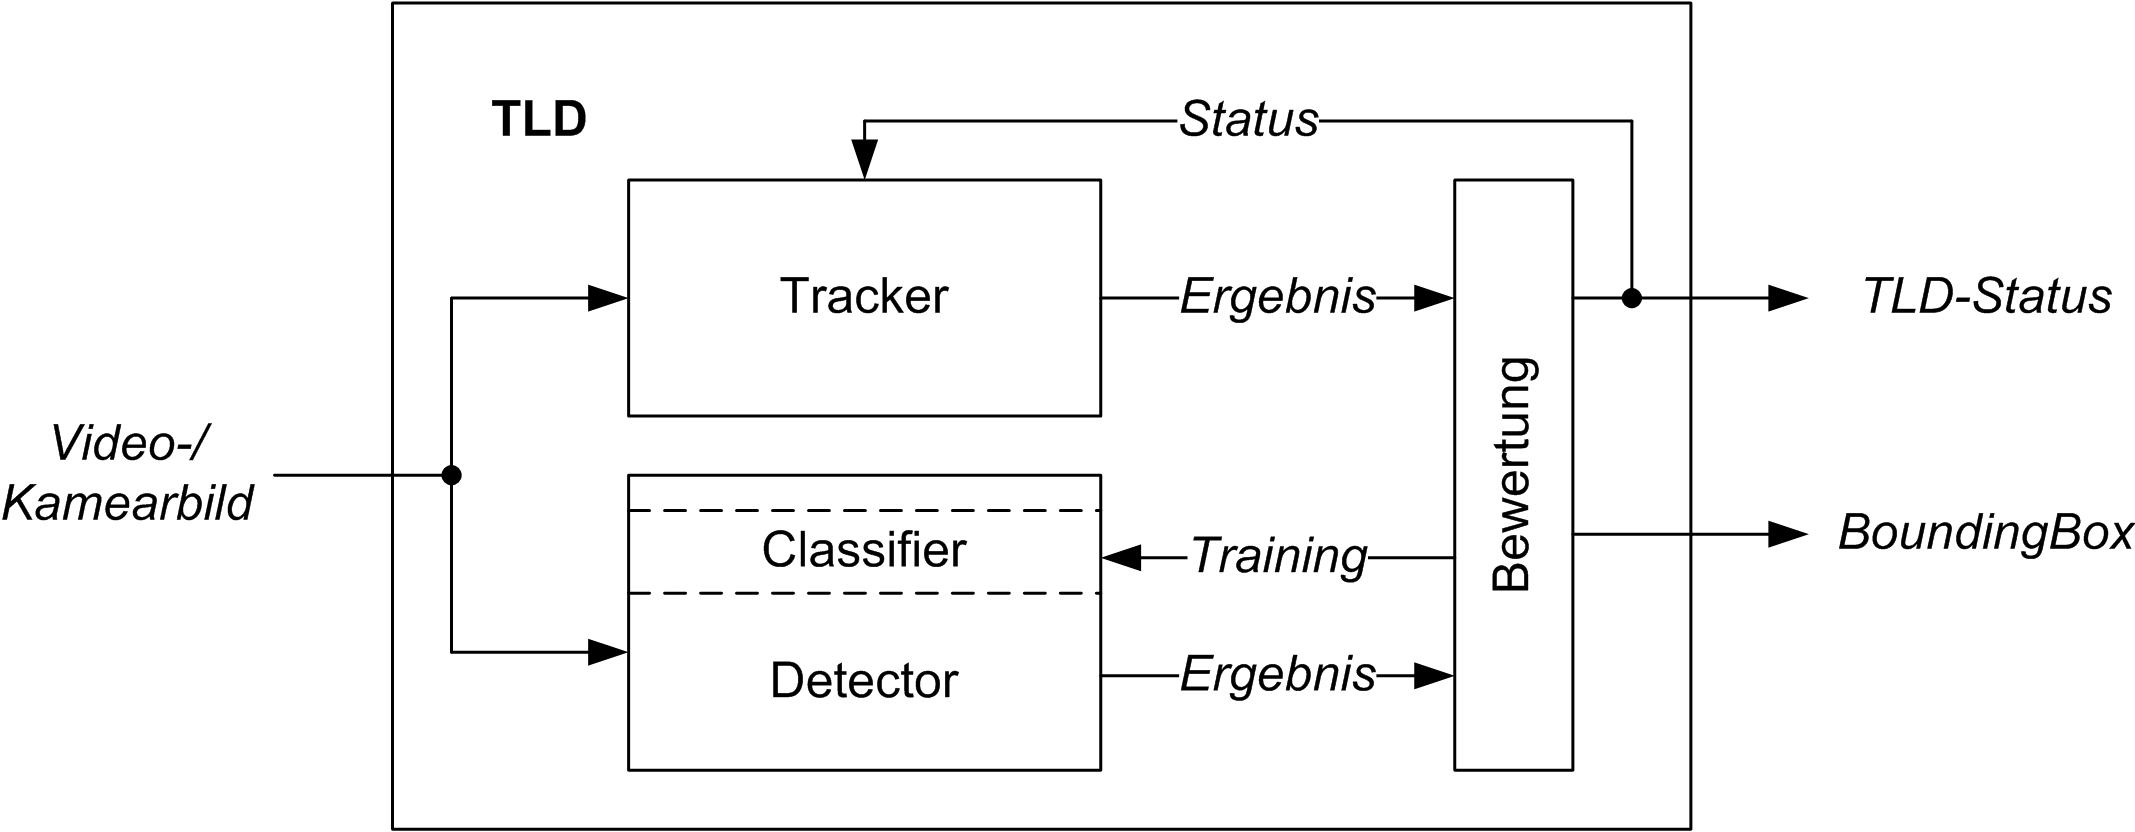
\includegraphics[scale=0.75]{../pictures/TLD-Framework.jpg}\caption{TLD-Schema}
\label{TLD-Schema}
\end{figure}

Als Implementationssprache wird C++ gewählt, weil sie aufgrund der re-lativen Hardwarenähe schnelle Prozesse und Programmabläufe ermöglicht. Zusätzlich ist durch OpenCV \cite{OCV} eine gut dokumentierte und umfangreiche Sammlung von C/C++-Algorithmen speziell für den Bereich der Computer Vision gegeben.

Im Anschluss zur Implementierung werden eine Reihe von Tests durchgeführt, die zu Beurteilung der Eignung von TLD für den speziellen Fall des Koptertrackings dienen. Es wird analysiert, welche Bedingungen zwingend gelten müssen, damit dieser Ansatz erfolgreich genutzt werden kann und unter welchen Umständen sich TLD nicht eignet.

\subsection{Aufbau der Arbeit}
Die Arbeit ist wie folgt gegliedert:

\paragraph{Kapitel 1}
  Das erste Kapitel stellt eine kurze Einführung in den Bereich der Computer Vision dar und leitet den speziellen Bereich der Objekterkennung ein. Wei-terhin wird die Zielsetzung der Arbeit definiert und der genutzte Algorithmus in Grundzügen vorgestellt.

\paragraph{Kapitel 2}
  Dieses Kapitel gibt einen kurzen Überblick zu verwandten Arbeiten und verschiedenen Ansätzen zur Lösung des Problems des machinellen Sehens. Unterschiedliche Paradigmen und deren Einsatzgebiete werden vergleichend vorgestellt.

\paragraph{Kapitel 3 }
  Hier erfolgt die genaue Beschreibung von TLD. Es werden ausführlich die theoretischen und mathematischen Hintergründe erläutert und der Algorithmus im Detail vorgestellt.

\paragraph{Kapitel 4}
	Im vierten Kapitel wird die C++-Implementierung in Ansätzen erläutert. Zusätzlich werden die verwendeten Testszenarien vorgestellt und die durchgeführten Tests beschrieben.

\paragraph{Kapitel 5}
	Den Abschluss dieser Arbeit bildet das fünfte Kapitel mit der Auswertung und Analyse der Testergebnisse sowie einer Reihe von Vorschlägen für etwaige Verbesserungen.

\paragraph{Anhang}
	Im Anhang werden die Klassensammlung { \em OpenCV} und die alternative Implementation { \em OpenTLD} vorgestellt, die zur Vervollständigung der Arbeit beigetragen haben. Außerdem befindet sich hier eine schematische Darstellung der wichtigsten Algorithmen, die in der TLD-Implementation zum Einsatz gekommen sind.